\documentclass{article}

% Pour utiliser toues les fonctions du clavier
\usepackage[utf8]{inputenc} % un package
\usepackage[T1]{fontenc}      % un second package

% Choix de la langue
\usepackage[francais]{babel}  % un troisième package
\setlength{\parindent}{0pt}

% Taille des marges
\usepackage[top=2.5cm, bottom=2cm, left=2.5cm, right=1.5cm]{geometry}

% Pour l'espace entre les lignes
\usepackage{setspace}
% Utilisation:
% Moyen:
% \begin{onehalfspace}
% \end{onehalfspace}
% Grand:
% \begin{doublespace}
% \end{doublespace}

% Changement des polices
\usepackage{charter}

% Pour afficher du code
\usepackage{verbatim}
\usepackage{moreverb}


\usepackage{titling}
\setlength{\droptitle}{-5em}   % This is your set screw

% Version 2
\usepackage{listings}

% Couleurs
\usepackage{color}
\usepackage[dvipsnames]{xcolor}
\usepackage{colortbl}

\title{Rapport Labo 3}
\author{Lucas \bsc{Bulloni} \&Bastien \bsc{Wermeille}}
%\date{10 Novembre 2017}

% En-têtes et pieds de pages
\usepackage{fancyhdr}
 
\pagestyle{fancy}
\fancyhf{}
\rhead{Lucas \bsc{Bulloni} \&Bastien \bsc{Wermeille}}
\lhead{Réseau et application.bib}
\chead{Rapport Labo 2}
\cfoot{\thepage}

% Package pour la légende de la table
\usepackage{caption}

% Package de multi-colonnes
\usepackage{multicol}

% Package pour les images
\usepackage{graphicx}

%bibliographie
\usepackage{csquotes}
%\usepackage{biblatex}
\usepackage[backend=bibtex]{biblatex}
%\addbibresource{biblio.bib}

% Pour les listes
\usepackage{enumitem}
\setlist[itemize]{topsep=0pt,after=\newline}

% package pour liens hypertexte
\usepackage{hyperref}

%\usepackage{minted}

% Début du document
\begin{document}

\maketitle

 

\section{Introduction}
 Le but de ce travail pratique est la découverte de techniques permettant de réaliser de la "Quality of Service" (QoS) sur un réseau simple. Ainsi que de tester ces dernières dans un environnement Netkit.

\subsection{Matériel et logiciel à disposition}
\begin{itemize}
	\item Un PC Linux avec NetKit
	\item Laboratoir netkit "qos"
\end{itemize}

\section{Méthodologie}

\subsection{Cas concret}
Grace au fichier lab.conf, nous pouvons déterminer la structure de réseau suivante:
\begin{figure}[h]
  \centering
  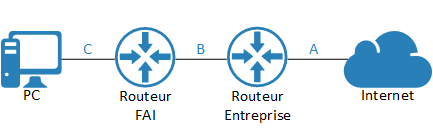
\includegraphics{./Structure.png}
  \caption{Structure du labo netkit}
  \label{fig:structure}
\end{figure}

Le démarrage du laboratoir NetKit "qos" nous permet d'accéder aux 4 périphériques précédement décrit:
\begin{itemize}
	\item PC
	\item Routeur Entreprise
	\item Routeur FAI
	\item Serveur Internet
\end{itemize}

%\begin{figure}[h]
%  \centering
%  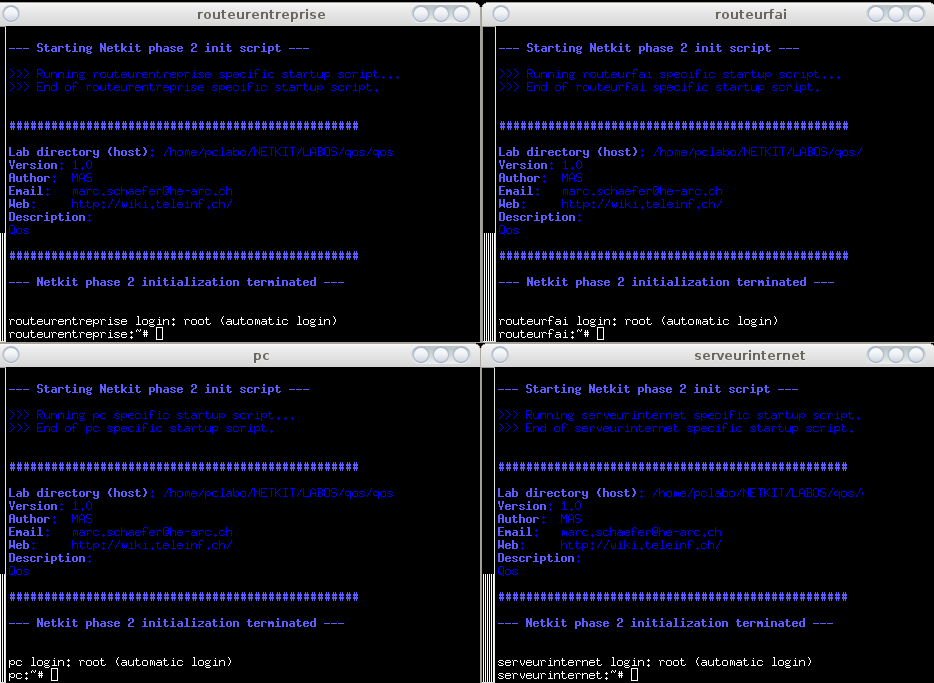
\includegraphics[width=\linewidth]{./captures/1-start.png}
%  \caption{Démarrage du labo netkit "QoS"}
%  \label{fig:qos}
%\end{figure}

\newpage
Une fois le laboratoire démarré, nous pouvons consulter le fichier routeurfai.startup :
\begin{figure}[h]
  \centering
  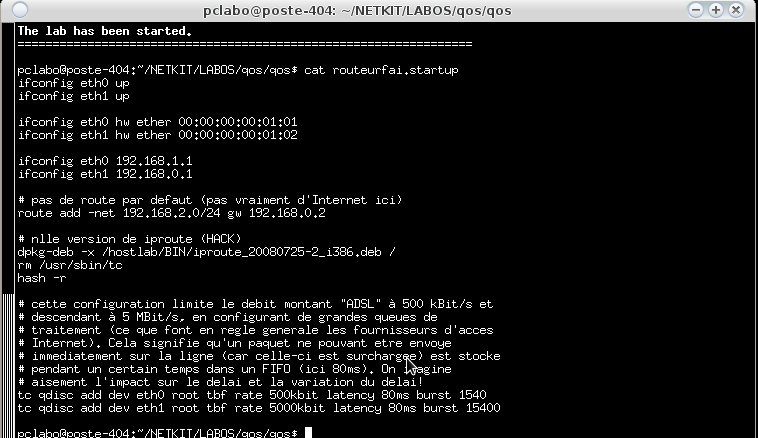
\includegraphics[width=\linewidth]{./captures/2-RouteurfaiStartup.png}
  \caption{Fichier de configuration "routeurfai.startup"}
  \label{fig:token-bucket}
\end{figure}

Ce fichier contient deux commandes qui influencent le traffic shapping, soient:
\begin{itemize}
\item \textit{tc qdist add dev eth0 root tbf rate 500kbit latency 80ms burst 1540}
\item \textit{tc qdist add dev eth1 root tbf rate 5000kbit latency 80ms burst 15400}
\end{itemize}

Grace à la commande "tcqdisc list", nous obtenons: 
\begin{figure}[h]
  \centering
  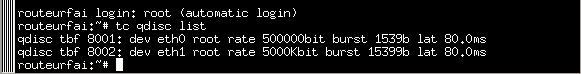
\includegraphics[width=\linewidth]{./captures/3-TokenBucket.png}
  \caption{Configurations Token Bucket}
  \label{fig:token-bucket}
\end{figure}

On peut y trouver deux paramètres, rate et latency, voici à quoi ils correspondent en comparaison avec le modèle du bacquet:
\begin{itemize}
\item rate -> débit standard
\item latency -> taille du bacquet
\end{itemize}

La configuration actuelle nous permet d'accéder à serveurinternet:
\begin{figure}[h]
  \centering
  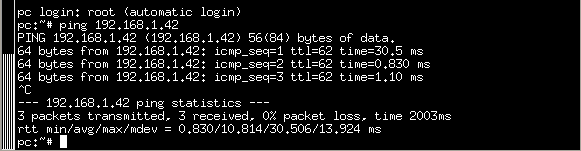
\includegraphics[width=\linewidth]{./captures/4-ping.png}
  \caption{Ping serveurinternet}
  \label{fig:token-bucket}
\end{figure}
\newpage

L'étape suivante a été d'évaluer les performances:

\begin{tabular}{|l|c|}
  \hline
   & Débit [Ko/s]\\
  \hline
  Débit montant & 49 \\
  Débit Descendant & 580 \\
  \hline
\end{tabular}
\\

ainsi que les pings:

\begin{tabular}{|l|c|}
  \hline
   & Temps [ms]\\
  \hline
  A vide & 1.19 \\
  avec débit descendant & 75 \\
  avec débit montant & 100 \\
  \hline
\end{tabular}
\\

TODO EVENTUELLEMENT AJOUTER CAPTURES + 

\subsubsection{Questions sur cette partie}
\textbf{a) Est-ce que les performances, chaque sens pris séparémment, correspond à celle prévue ?}\\
Oui, 
\\

\textbf{b) si vous faites des transferts dans les deux sens, qu'observez-vous au niveau des débits ?}\\
Bous avons effectué un test en mesurant le débit dans les deux directions en même temps:\\
\begin{tabular}{|l|c|}
  \hline
   & Débit [Ko/s]\\
  \hline
  Débit montant & 45 \\
  Débit Descendant & 516 \\
  \hline
\end{tabular}
\\

On constate que les deux débits sont plus petits que ceux mesurés indépendemment, celà s'explique par le fait que chaque message reçu dans un sens nécessite une confirmation qui va prendre du débit dans le sens opposé.
\\

\textbf{c) Qu'observez-vous si vous faites des ping simultanément à des transferts ?}\\
Plus de traffic car TODO EXPLIQUER POURQUOI

\subsubsection{Partie spécifique au rapport}
Grace au script, nous avons généré le graph de latence, une fois sans traffic:
\begin{figure}[h]
  \centering
  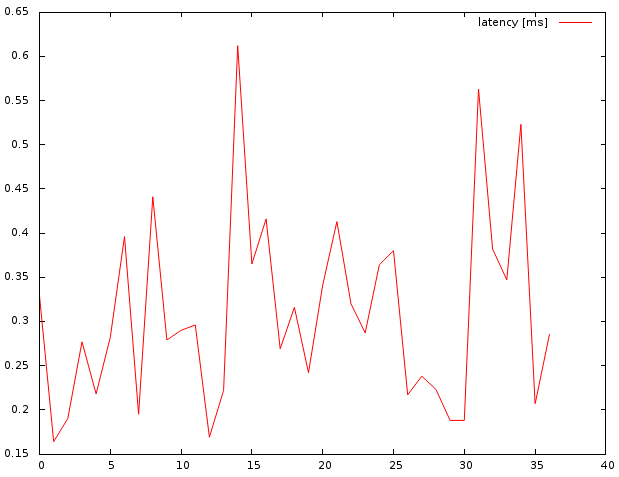
\includegraphics[width=\linewidth]{./captures/6-plot.png}
  \caption{Configurations Token Bucket}
  \label{fig:token-bucket}
\end{figure}

Puis la seconde fois avec du traffic full-duplex afin de diminuer l'effet aléatoire losrqu'il n'y a pas de traffic et que la variance varie beaucoup en très peu de temps:
\begin{figure}[h]
  \centering
  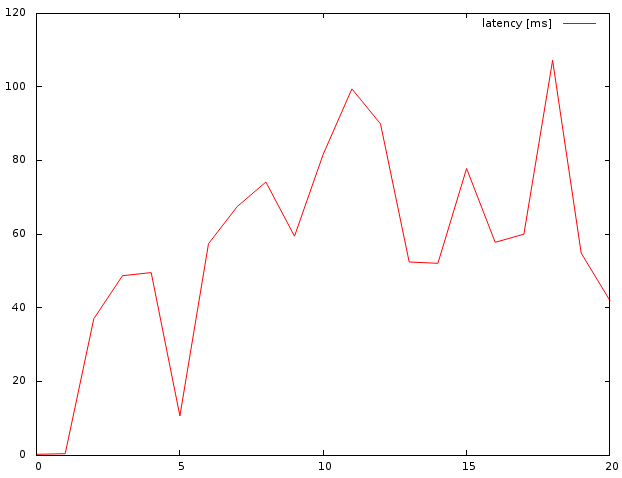
\includegraphics[width=\linewidth]{./captures/6-plot-fullduplex.png}
  \caption{Configurations Token Bucket}
  \label{fig:token-bucket}
\end{figure}

Nous avons également simulé des flux udp et effectué un ping:\\
TODO IL FUDRAIT QU'ON AI UNE CAPTURE DE LA COMMANDE UDP

\begin{figure}[h]
  \centering
  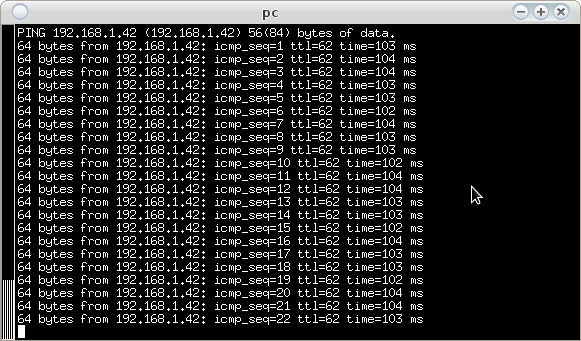
\includegraphics[width=\linewidth]{./captures/10-udp.png}
  \caption{ping durant traffic upd}
  \label{fig:token-bucket}
\end{figure}


\subsection{Traffic Shaping Simple}



\subsection{Marquage du trafic classifié}

\subsection{Classification et traffic shaping hiérarchique}

\subsection{Traffic descendant}

\section{Questions de base}

\subsection*{1 : Expliquer en quelques mots le principe l'algorithme de régulation TCP}

Certains routeur vont marquer les pacquets lorsqu'ils s'apprêtent à subir une congestion, ce système s'appelle l'ECN (Explicit Congestion Notification). Mais ce système mise sur le fait que les d'autres routeurs implément ce système. \cite{cours}\\

Les paquets marqués vont indiquer au client qu'il doit diminuer son débit.

\subsection*{2 : Pourquoi un MTU plus faible peut améliorer la QoS?}

Un MTU plus faible va baisser l'efficacité de la communication mais va améliorer le temps de réponse.
\begin{enumerate}
\item Problème de partage des trames
\item Guigge de phase très variable
\item Baisse de l'efficacité mais augmente le temps de réponse
\end{enumerate}

\subsection*{3 : Que doit faire un opérateur lorsqu'il remarque des bits TOS et DIFFSERV ?}

Lorsqu'un opérateur remarque des bits TOS \cite{ToS} et DIFFSERV \cite{DiffServ} chez un client qui n'a pas de qualité de service dans sa prestation veut dire qu'il essaye de tricher.\\

L'opérateur peut alors faire 2 choses différentes selon sa politique envers ses clients qui essayent de tricher : 

\begin{itemize}
 	\item Jeter tous les paquets
 	\item Ignorer ces bits et les supprimer de tous les paquets
\end{itemize}

\subsection*{4 : Comment diminuer la vitesse du sens descendant en modifiant celle du sens montant?}

Il y a deux possiblités. La première est de réduire la vitesse du débit montant de cette connexion, ce qui aura pour effet d'également de réduire la vitesse du sens descendant, car les paquêts metteront plus de temps à atteindre leur destination et leur reponse sera donc envboyer plus tard.\\

La deuxième solution  est de supprimer des paquets de confirmations. L'émetteur attendra alors jusqu'au timeout et va ré-émettre le paquet par la suite. La fenêtre passera également moins rapidement aux paquets suivant puisque certains paquets n'auront pas été confirmés.

\subsection*{5 : Le sens montant est saturé, comment assuer un bon débit descendant}

Il serait possible de grouper les confirmations (ACK) comme le fait go back-n\cite{GoBackN} ou alors en faisant de la QoS et en priorisant le traffic montant et les confirmations.\\

Si on priorise le traffic montant alors passera plus facilement outre la saturation et les confirmations du serveur seront en traffic descendant qui lui, n'est pas saturé.


\subsection*{6 : Pourquoi gérer le traffic shaping seulement sur routeurentreprise produit de bon résultat mais n'est toujours pas suffisant?}

Le première raison est que le routeur entreprise ne peut gérer que le traffic propre à son sous-réseau et non tous les clients connectés à routeur FAI. Le routeur FAI aura donc un traffic beaucoup plus important et la QoS sera donc plus utile sur cette partie du réseau.\\

Mais le faire sur le routeur de l'entreprise permet déjà d'avoir une priorisation par rapport au traffic de l'entreprise et donc d'avoir un résultat qui peut-être satisfaisant si le routeur FAI ne subit très peu de congestion.

\subsection*{7 : Quelle queue est recommendé pour garantir un traitement équitables des données? Est-ce que le Token Bucket répond à ses besoin ?}

Une queue de type SFQ \cite{SFQ} est recommendé pour garantir un traitement plus équitables des données.\\

Un baquet ne serait pas adapté car ce système ce contente de supprimer tous les paquets lorsqu'il est en surcharge \cite{Bucket}


\section{Questions rapport}

\subsection*{1 : Qu'est ce que le routage de la patate chaude et à quoi sert-il dans un réseau surchargé?}

- Il envoie tout ce qu'il reçoit et s'il y a un routeur qui est surchargé, il envoie le paquet à un autre routeur

\subsection*{2 : Avec quel outil peut-on évaluer le nombre de paquets reçus en désordre?}

- Wireshark avec des filtres

\subsection*{3 : Proposer une répartition de débit entre classes plus logique dans un réseau réel}

- Prioriser le tcp

\subsection*{4 : Conception d'un baquet}

%\begin{minted}{python}

%\end{minted}


\section{Conclusion}


%\bibliography{biblio.bib}{}
%\bibliographystyle{plain}

\printbibliography 

\end{document}
